\documentclass[a4paper,11pt,dvipdfmx]{jsarticle}


% 数式
\usepackage{amsmath,amsfonts}
\usepackage{bm}
% 画像
% \documentclass{article}
\usepackage[dvipdfmx]{graphicx}
\usepackage{circuitikz}
\usepackage{amsmath,amssymb}
\usepackage{siunitx}
\usepackage{float}
\usepackage{tikz}
\usepackage{askmaps}
\usepackage{multirow}
\usepackage{bigstrut}

\newcommand{\Figure}[4]{
  \begin{figure}[H]
    \centering
    \includegraphics[width=#1\linewidth]{#2}
    \caption{#3}
    \label{fig:#4}
  \end{figure}
}

\begin{document}

\begin{table}[b]
  \centering
  \begin{tabular}{|c|c|}
    \hline
    報告者     & 22120 222 塚田 勇人 \\
    \hline
    共同実験者 & 22192 234 山本 悠介  \\ & 22060 211 古城 隆人\\
    \hline
    担当者     & 楡井 雅巳 \\
              &  藤澤 義範\\
    &力丸 彩奈\\
    &村田 雅彦\\
    &富岡 雅弘\\
    \hline
    実験年月日 & 2024年9月27日 天気:曇り 気温:26.2℃ 湿度68\verb#%#\\
    & 2024年10月4日 天気:曇り 気温:25.9℃ 湿度74\verb#%#\\
    & 2024年10月11日 天気:晴れ 気温:22.1℃ 湿度53\verb#%#\\
    & 2024年10月17日 天気:晴れ 気温:25.0℃ 湿度51\verb#%#\\
    \hline
    提出期限   & 2024年10月24日 23:59  \\
    \hline
    提出日     & \today              \\
    \hline
  \end{tabular}
\end{table}


\title{デコーダ回路の設計と制作}
\author{塚田 勇人}
\date{\today}
\maketitle

\newpage
\section{目的}
電子天秤の制作を行うにあたり、値を表示させるために7セグメントLED1の表示回路を設計し、作成する。それにより
論理設計の理解を深め、基本的な論理回路を組み合わせる技術を学ぶ。また、実際に配線し回路を作成することで、汎用ロジックICや
ブレッドボードなどのハードウェアについても学ぶ。
セレクタ回路から3bitの信号を受け取る。
\section{原理}
実際に回路の制作を行うにあたって使用する部品と動作原理を説明する。
\subsection{デコーダ回路}
デコーダ回路とは複数bitの2進数符号に対応する1つの出力にアクセスする回路である\cite{Khokasho}。
\subsection{ブレッドボード}
ブレッドボードとは電子回路を制作するための部品である。ブレッドボードはジャンパ線を使用して部品を接続することが出来る。
今回はデコード回路の作成のため用いる。
ブレッドボードの内部構造を図\ref{fig:breadboard}に示す。\\
\begin{figure}[H]
  \centering
  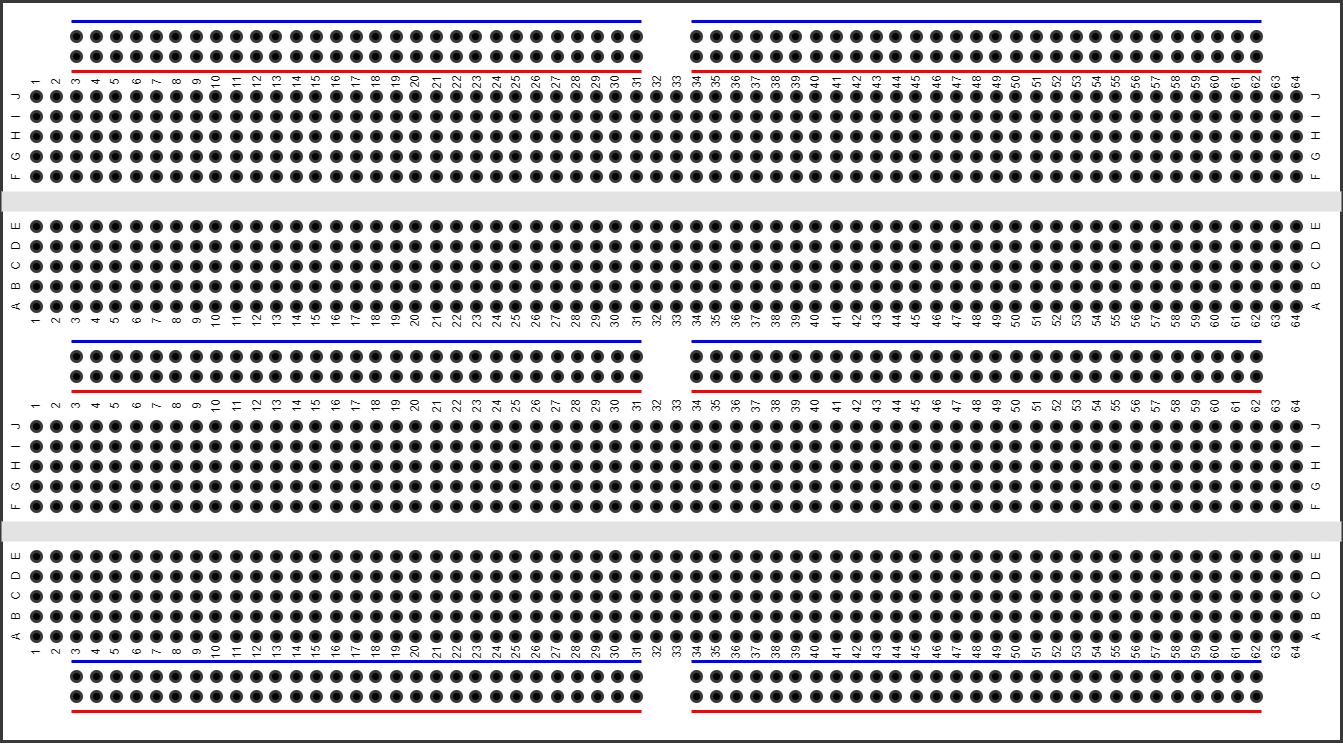
\includegraphics[width=10cm]{./images/breadboard.drawio.png}
  \caption{ブレッドボードの内部構造}
  \label{fig:breadboard}
\end{figure}
ブレッドボードは図\ref{fig:breadboard}のように、縦に7列のピンがある。このピンは縦に繋がっている。
また、縦の列は電源が繋がっている。
ブレッドボードの横の列は繋がっていない。そのため、横の列にはジャンパ線を使用して繋げる必要がある。
ブレッドボードの中央には溝があり、この溝にICを挿入することが出来る。ICのピンは縦に繋がっているため、
ICを挿入するときは必ず溝を挟むように、注意が必要である。

\subsection{トグルスイッチ}
トグルスイッチとは、回路のオンオフを切り替えたり、流れる信号の変更を行うためのスイッチである。本実験で用いるトグルスイッチは、$EN$の信号のHighとLowを切り替える。
トグルスイッチがオフになったときは$\overline{EN}$は常に1となるので、セグメントは点灯しない。

\subsection{7セグメントLED}
7セグメントLEDとは7つのLEDを組み合わせたもので、数字を表示させる用途で使用する。7つのLEDはそれぞれaからgまでの名前が
ついており、それぞれのLEDを点灯させることで数字を表示させる。なお、このレポート
では以降7セグメントLEDのことを7セグLEDと略すことにする。
7セグLEDの略図を図\ref{fig:7seg}に示す。
\begin{figure}[H]
  \centering
  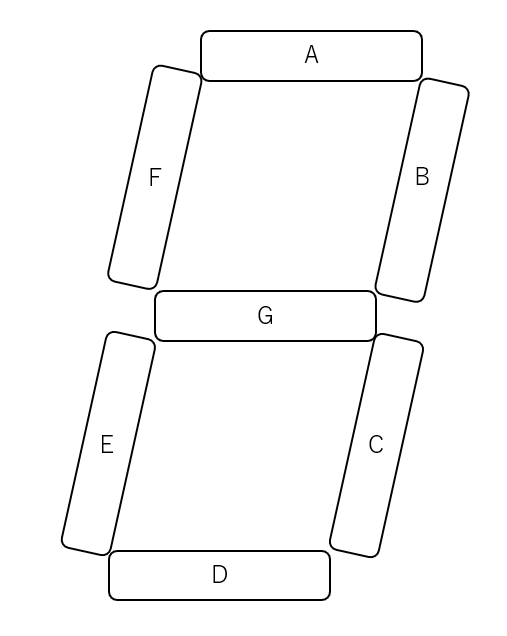
\includegraphics[width=5cm]{./images/7seg.png}
  \caption{7セグLEDの略図}
  \label{fig:7seg}
\end{figure}
基本的に一番上から時計回りにaからgまでのLEDが配置されている。\\
7セグLEDはアノードコモンとカソードコモンの2種類がある。その二つについて説明する。
\subsubsection{アノードコモン}
\label{sec:anode}
アノードコモンとは、7セグメントLEDのアノードが共通になっているタイプである。アノードコモンの場合、アノードに
電圧をかけることで、セグメントが点灯する。

\subsubsection{カソードコモン}
カソードコモンとは、7セグメントLEDのカソードが共通になっているタイプである。カソードコモンの場合、カソードに
電圧をかけることで、セグメントが点灯する。
\\\\
今回使用する7セグLEDはアノードコモンである。
7セグLEDは10個のピンがある。ピン配置を図\ref{fig:7segpin}に示す。
\begin{figure}[H]
  \centering
  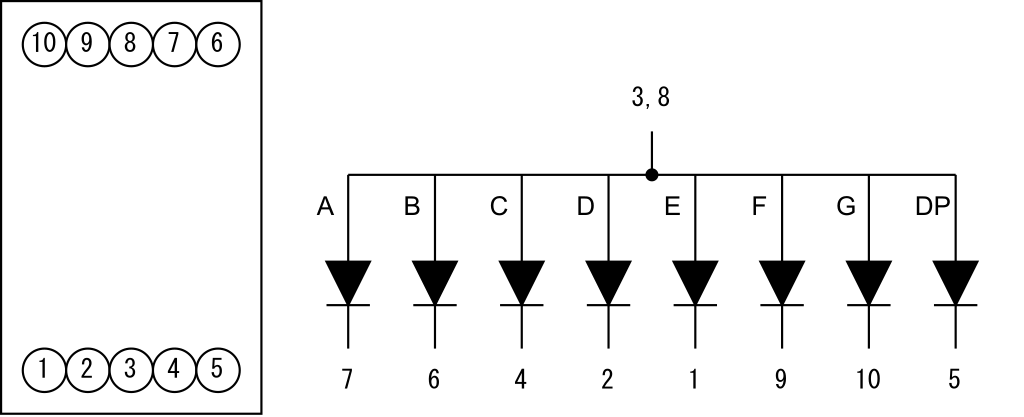
\includegraphics[width=10cm]{./images/7segpin.png}
  \caption{7セグメントLEDのピン配置}
  \label{fig:7segpin}
\end{figure}
左下のピンから反時計回りに1から10までのピンがあり、3,8がアノードでそれ以外がカソードに接続している。


\subsection{汎用ロジックIC}
汎用ロジックICは論理演算を行うことが出来る回路部品である。今回は2進数の情報を基に7セグLEDの光らせ方を制御するのに
使用する。\\
論理演算ではAND / ORなどがある。例えばAND演算では2本の入力がHIGH($+5V$)の時に出力がHIGHになる。これはどちらも1で
あるためである。論理回路の入力と出力を示したものを真理値表という。表の列の数だけ変数があり、入力/出力、場合によっては内部の状態を示す。
AND、OR、NOT、XORの真理値表を表\ref{tab:logic}に示す。
\begin{table}[H]
  \centering
  \caption{論理演算の真理値表}
  \begin{tabular}{|c|c|c|c|c|c|c|}
    \hline
    A & B & AND & OR & NOT (A) & NOT (B) & XOR \\
    \hline
    0 & 0 & 0 & 0 & 1 & 1 & 0 \\
    0 & 1 & 0 & 1 & 1 & 0 & 1 \\
    1 & 0 & 0 & 1 & 0 & 1 & 1 \\
    1 & 1 & 1 & 1 & 0 & 0 & 0 \\
    \hline
  \end{tabular}
  \label{tab:logic}
\end{table}
今回ではA、Bが入力で、AND、OR、NOT、XOR、が出力である。
この0と1はそれぞれLOW($GND$)、HIGH($+5V$)を示している。\\
ICでは内部の特徴に違いがあり、それを名前で表している。今回使用するICについてそれぞれ説明する。
\subsubsection{SN74LS04N}
SN74LS04Nとは、NOTゲートを6つ内蔵したICである。NOTゲートは、入力された信号を反転させる回路である。
SN74LS04Nのピンアサインを図\ref{fig:NOT}に示す。
\Figure{0.4}{./images/74LS04.png}{SN74LS04Nのピンアサイン}{NOT}

\subsubsection{SN74LS08N}
SN74LS08Nとは、ANDゲートを4つ内蔵したICである。ANDゲートは、入力された信号がすべてHighのときにHighを出力する回路である。
SN74LS08Nのピンアサインを図\ref{fig:AND}に示す。
\Figure{0.4}{./images/74LS08.png}{SN74LS08Nのピンアサイン}{AND}

\subsubsection{SN74LS32N}
SN74LS32Nとは、ORゲートを4つ内蔵したICである。ORゲートは、入力された信号のうち1つでもHighがあればHighを出力する回路である。
SN74LS32Nのピンアサインを図\ref{fig:OR}に示す。
\Figure{0.4}{./images/74LS32.png}{SN74LS32Nのピンアサイン}{OR}

\subsubsection{SN74LS86N}
SN74LS86Nとは、XORゲートを4つ内蔵したICである。XORゲートは、入力された信号が異なるときにHighを出力する回路である。
SN74LS86Nのピンアサインを図\ref{fig:XOR}に示す。
\Figure{0.4}{./images/74LS86.png}{SN74LS86Nのピンアサイン}{XOR}

% ICには論理回路に入出力があるように、入出力するための端子がある。その内部の構造として、出力端子を説明する。
% ICの内部は複数のトランジスタで構成されている。
% トランジスタとはスイッチのようなもので、ベースとエミッタの電位差によってコレクタとエミッタ間の電流を制御できる。
% トランジスタにはNPN型とPNP型の2種類があるが今回はNPN型で説明を行う。
% NPN型トランジスタの特性はベースとエミッタ間に電流が流れる。
% 要は電位がベースのほうが大きくなるとコレクタからエミッタにかけて電流が流れる。\\
% 図\ref{fig:transistor}にトランジスタの特性を示す。
% \begin{figure}[H]
%   \centering
%   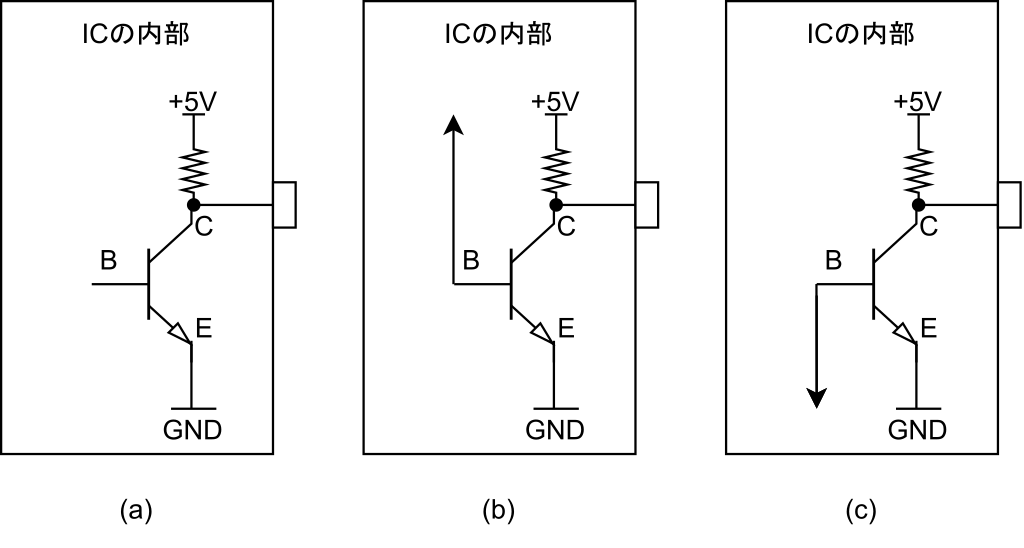
\includegraphics[width=10cm]{./images/trans.png}
%   \caption{トランジスタの特性}
%   \label{fig:transistor}
% \end{figure}

% 図 \ref{fig:transistor}ではBをベース、Cをコレクタ、Eをエミッタとしている。\\
% 図 \ref{fig:transistor}(a)はICの出力端子の一個前のイメージである。右側の四角いでっぱりが出力端子で、内部に
% 書かれているものが出力の一個前のトランジスタである。\\
% 図 \ref{fig:transistor}(b)(c)は出力端子のイメージである。(b)では、ベースとエミッタ間に電流が流れるとコレクタと
% エミッタ間に電流が流れる。そのため出力端子に電流が流れないため、出力はLOWとなる。この出力の先に電流が流れるかも
% しれないが、この先に接続するICの内部抵抗よりもトランジスタの抵抗のほうが小さいのでエミッタに電流が流れる。\\
% (c)では、ベースとエミッタが同じ電位にあるため、コレクタからエミッタにかけて電流が流れない。そのため出力端子の先に違う
% 電位があれば電流が流れる。IC内部で発生するこれらの電流のことを前者をシンク電流、後者をソース電流という。\\
% ICによってシンク電流、ソース電流の値が異なるのでデータシートで確認を行い、電子回路を組むことが出来るのかを把握する
% 必要がある。例えば今回ではアノードコモンのLEDを制御するため出力端子にLEDのカソードを接続し、シンク電流を流すことで
% LEDを光らせる。そのため、$I_{ol}$の電流を確認する必要がある。$I_{ol}$はシンク電流、$I_{oh}$はソース電流である。
% 汎用ロジックICではピン番号が同じように命名されている。\\
% 今回使用するICは74LS04(NOT)、74LS08(AND)、74LS32(OR)、74LS86である。いずれも14ピンのDIP型のICである。
% DIPとはDual Inline Packageの略称であり、パッケージの表面にくぼみがあるのが特徴である。このくぼみがあるほうを表、
% 端子が出てるほうが裏である。表の状態でくぼみを上にした時に、左上から反時計回りに1から14までの数字が命名されている。
% 74シリーズでは7番に$GND$、14番に$+5V$を接続する。それ以外の端子は入出力端子である。

\subsection{ピンヘッダ}
ピンヘッダとは、ブレッドボードにICを挿入するための部品である。ピンヘッダはICのピンとブレッドボードのピンを繋ぐために
使用する。今回は$2\times 7$ピン、端子間距離が$2.54mm$のT字コネクタのピンヘッダを用いる。
これは一般的なピンヘッダの端子間距離であり今回使用するブレッドボードもこの端子間距離である。

% \subsection{カルノー図}
% デコーダ回路は複雑な回路になるため、論理式を立てる。論理式は真理値表を基に作成することが出来るが、複雑な回路になると
% 論理式が複雑になる。そのため、カルノー図を使用することで論理式を簡単に作成することが出来る。
% カルノー図は出力の数だけ表を作成し、論理式の作成を行う。表 \ref{tab:karno}にカルノー図の例を示す。
% これは7セグLEDのB端子用のカルノー図である。真理値表からここから論理式の計算を行う。
% まず初めに、表の中で1の部分をグループ化を行う。その後、グループ化した部分を論理式に変換する。
% グループ化したものを\ref{fig:karno1}に示す。これを論理式に変換すると 数式\eqref{eq:b-output} となる。
% これを簡単にすると、 \eqref{eq:b-output1} となる。6個の論理素子の使用から、3個の論理素子の使用に減らすことが出来る。
% カルノー図から論理式を立てて簡略化してないように見えるが真理値表から論理式を立てた場合、出力がHIGHの量の数 $\times$  3個の論理素子が必要になる式になる。
% そのため今回ではカルノー図にする前は30個の論理素子が必要であった。

% \begin{figure}[htbp]
%   \begin{minipage}[b]{0.49\columnwidth}
%   \centering
%   \askmapiv{\(B\)}{{\(EN\)}{\(IN_0\)}{\(IN_1\)}{\(IN_2\)}}{}{11111111{\phantom{0}}{\phantom{0}}{\phantom{0}}{\phantom{0}}{\phantom{0}}11{\phantom{0}}}{}
%   \caption{\(B\)のカルノー図}
%   \label{}
%   \end{minipage}
%   \begin{minipage}[b]{0.49\columnwidth}
%   \centering
%   \askmapiv{\(B\)}{{\(EN\)}{\(IN_0\)}{\(IN_1\)}{\(IN_2\)}}{}{11111111{\phantom{0}}{\phantom{0}}{\phantom{0}}{\phantom{0}}{\phantom{0}}11{\phantom{0}}}
%   {
%    \color{black}\put(0.85,2){\oval(1.8,3.8)}
%    \color{black}\put(1.9,2.5){\oval(1.8,0.8)}
%    \color{black}\put(1.9,0.5){\oval(1.8,0.8)}
%   }
%   \caption{\(B\)のカルノー図}
%   \label{fig:karno1}
%   \end{minipage}
% \end{figure}


\section{実験方法}
デコーダーの真理値表を作成し、それに基づいて論理式を作成する。そして論理式を基にカルノー図を用いて簡単化し、回路図を
作成する。作成した回路図をもとに配線をし、デコーダー回路を作成する。

\subsection{実験に用いた機器}
今回の課題に用いた機器や電子部品について表\ref{tab:equipment}と表\ref{tab:electronicParts}に示す。

\begin{table}[H]
  \caption{実験に用いた機器}
  \centering
  \begin{tabular}{c|c|c}
    \hline
    器具名         & 製造元    & 計器番号    \\
    \hline \hline
    ブレッドボード & Sunhayato & SRH-32      \\
    \hline
    マルチテスター & NISHIZAWA & MODEL 5220  \\
    \hline
    ACアダプタ     & Fksystem  & GF12-US0520 \\
    \hline
  \end{tabular}
  \label{tab:equipment}
\end{table}


\begin{table}[H]
  \caption{実験に用いた電子部品}
  \centering
  \begin{tabular}{c|c|c|c}
    \hline
    部品名         & 諸元                & 個数 & 部品記号 \\
    \hline \hline
    抵抗           & 300Ω±5\verb|%| & 7    & R1~R7   \\
    \hline
    7セグメントLED & LN516RA             & 1    & DIS1     \\
    \hline
    集積回路(IC)1  & SN74LS04N           & 1    & IC1      \\
    \hline
    集積回路(IC)2  & SN74LS08N           & 2    & IC2~IC4 \\
    \hline
    集積回路(IC)3  & SN74LS32N           & 2    & IC5~IC7 \\
    \hline
    集積回路(IC)4  & SN74LS86N           & 1    & IC8      \\
    \hline
    ピンヘッダ     & 2*7ピン             & 1    & PH1      \\
    \hline
    トグルスイッチ & ON-OFF              & 1    & SW1      \\
    \hline
  \end{tabular}
  \label{tab:electronicParts}
\end{table}

\subsection{論理式の作成}
デコーダ回路の回路図を作成するために真理値表を作成して論理式を
立てていく。作成した真理値表を表\ref{tab:truth}に示す。
この真理値表を元にカルノー図の作成を行う。
\begin{table}[H]
  \centering
  \caption{真理値表}
  \begin{tabular}{|c|c|c|c|c|c|c|c|c|c|c|}
    \hline
    $EN$ & $IN_2$ & $IN_1$ & $IN_0$ & $A$ & $B$ & $C$ & $D$ & $E$ & $F$ & $G$ \\
    \hline
    0 & * & * & * & 1 & 1 & 1 & 1 & 1 & 1 & 1 \\
    1 & 0 & 0 & 0 & 0 & 0 & 0 & 0 & 0 & 0 & 1 \\
    1 & 0 & 0 & 1 & 1 & 0 & 1 & 1 & 1 & 1 & 0 \\
    1 & 0 & 1 & 0 & 0 & 0 & 0 & 0 & 0 & 1 & 0 \\
    1 & 0 & 1 & 1 & 0 & 0 & 0 & 0 & 1 & 1 & 0 \\
    1 & 1 & 0 & 0 & 1 & 0 & 0 & 1 & 1 & 0 & 0 \\
    1 & 1 & 0 & 1 & 0 & 1 & 0 & 0 & 1 & 0 & 0 \\
    1 & 1 & 1 & 0 & 0 & 1 & 0 & 0 & 0 & 0 & 0 \\
    1 & 1 & 1 & 1 & 0 & 0 & 0 & 1 & 1 & 0 & 1 \\
    \hline
  \end{tabular}
  \label{tab:truth}
\end{table}
この真理値表をもとに端子$A$から$G$の論理式を作成する。論理式を作成し
簡単化する。
\subsubsection{端子A}
\label{sec:a}
7セグLEDの端子$A$を図\ref{fig:karnoA}に示す。これを基に論理式を作成すると、数式\eqref{eq:a-output}となる。
これを簡単にすると、数式\eqref{eq:a-output1}となる。
\begin{figure}[H]
  \centering
    \askmapiv{\(A\)}{{\(EN\)}{\(IN_2\)}{\(IN_1\)}{\(IN_0\)}}{}{11111111{\phantom{0}}1{\phantom{0}}{\phantom{0}}1{\phantom{0}}{\phantom{0}}{\phantom{0}}}
    {
    \color{black}\put(0.85,2){\oval(1.8,3.8)}
    \color{black}\put(1.9,3.5){\oval(1.8,0.8)}
    \color{black}\put(3.9,2.5){\oval(1.8,0.8)[l]}
    \color{black}\put(-0.1,2.5){\oval(1.8,0.8)[r]}
    }
    \caption{\(A\)のカルノー図}
    \label{fig:karnoA}
\end{figure}

\begin{align}
  A &= \overline{EN} + \overline{IN_2} \cdot \overline{IN_1} \cdot IN_0 + IN_2 \cdot \overline{IN_1} \cdot \overline{IN_0} \label{eq:a-output}\\
  &= \overline{EN} + \overline{IN_2} \cdot ( IN_2 \oplus IN_0) \label{eq:a-output1}
\end{align}

\subsubsection{端子B}
7セグLEDの端子$B$を図\ref{fig:karnoB}に示す。これを基に論理式を作成すると、数式\eqref{eq:b-output}となる。
これを簡単にすると、数式\eqref{eq:b-output1}となる。
\begin{figure}[H]
  \centering
    \askmapiv{\(B\)}{{\(EN\)}{\(IN_2\)}{\(IN_1\)}{\(IN_0\)}}{}{11111111{\phantom{0}}{\phantom{0}}{\phantom{0}}{\phantom{0}}{\phantom{0}}11{\phantom{0}}}
    {
    \color{black}\put(0.85,2){\oval(1.8,3.8)}
    \color{black}\put(1.9,2.5){\oval(1.8,0.8)}
    \color{black}\put(1.9,0.5){\oval(1.8,0.8)}
    }
    \caption{\(B\)のカルノー図}
    \label{fig:karnoB}
\end{figure}

\begin{align}
  B &= \overline{EN} + IN_0 \cdot \overline{IN_1} \cdot IN_2 + \overline{IN_0} \cdot IN_1 \cdot IN_2 \label{eq:b-output}\\
  &= \overline{EN} + IN_2 \cdot (IN_0 \oplus IN_1  ) \label{eq:b-output1}
\end{align}

\subsubsection{端子C}
7セグLEDの端子$C$を図\ref{fig:karnoC}に示す。これを基に論理式を作成すると、数式\eqref{eq:c-output}となる。\\
\begin{figure}[H]
  \centering
  \askmapiv{\(C\)}{{\(EN\)}{\(IN_2\)}{\(IN_1\)}{\(IN_0\)}}{}{11111111{\phantom{0}}1{\phantom{0}}{\phantom{0}}{\phantom{0}}{\phantom{0}}{\phantom{0}}{\phantom{0}}}
  {
   \color{black}\put(0.85,2){\oval(1.8,3.8)}
   \color{black}\put(3.9,2.5){\oval(1.8,0.8)[l]}
   \color{black}\put(-0.1,2.5){\oval(1.8,0.8)[r]}
  }
  \caption{\(C\)のカルノー図}
  \label{fig:karnoC}
\end{figure}

\begin{align}
  C &= \overline{EN} + \overline{IN_2} \cdot IN_1 \cdot \overline{IN_0}\label{eq:c-output}
\end{align}

\subsubsection{端子D}
7セグLEDの端子$D$を図\ref{fig:karnoD}に示す。これを基に論理式を作成すると、数式\eqref{eq:d-output}となる。
これを簡単にすると、数式\eqref{eq:d-output1}となる。\\
\begin{figure}[H]
    \centering
    \askmapiv{\(D\)}{{\(EN\)}{\(IN_2\)}{\(IN_1\)}{\(IN_0\)}}{}{11111111{\phantom{0}}1{\phantom{0}}{\phantom{0}}1{\phantom{0}}{\phantom{0}}1}{
      \color{black}\put(0.85,2){\oval(1.8,3.8)}
      \color{black}\put(3.9,2.5){\oval(1.8,0.8)[l]}
      \color{black}\put(-0.1,2.5){\oval(1.8,0.8)[r]}
      \color{black}\put(1.9,3.5){\oval(1.8,0.8)}
      \color{black}\put(1.9,1.5){\oval(1.8,0.8)}
    }
    \caption{\(D\)のカルノー図}
    \label{fig:karnoD}
\end{figure}

\begin{align}
  D &= \overline{EN} + IN_2 \cdot IN_1 \cdot IN_0 + IN_2 \cdot \overline{IN_1} \cdot \overline{IN_0} + \overline{IN_2} \cdot \overline{IN_1} \cdot IN_0\label{eq:d-output}\\
  &= \overline{EN} + IN_1 \cdot (IN_2 \oplus IN_0) + IN_2 \cdot IN_1 \cdot IN_0\label{eq:d-output1}
\end{align}

\subsubsection{端子E}
7セグLEDの端子$E$を図\ref{fig:karnoE}に示す。これを基に論理式を作成すると、数式\eqref{eq:e-output}となる。\\
\begin{figure}[H]
  \centering
    \askmapiv{\(E\)}{{\(EN\)}{\(IN_2\)}{\(IN_1\)}{\(IN_0\)}}{}{11111111{\phantom{0}}1{\phantom{0}}111{\phantom{0}}1}{
      \color{black}\put(0.85,2){\oval(1.8,3.8)}
      \color{black}\put(1.9,2.0){\oval(3.8,1.8)}
      \color{black}\put(1.9,3.0){\oval(1.8,1.8)}
    }
    \caption{\(E\)のカルノー図}
    \label{fig:karnoE}
\end{figure}

\begin{align}
  E &= \overline{EN} + IN_0 + \overline{IN_1} \cdotp IN_2\label{eq:e-output}
\end{align}

\subsubsection{端子F}
7セグLEDの端子$F$を図\ref{fig:karnoF}に示す。これを基に論理式を作成すると、数式\eqref{eq:f-output}となる。
これを簡単にすると、数式\eqref{eq:f-output1}となる。\\
\begin{figure}[H]
  \centering
    \centering
    \askmapiv{\(F\)}{{\(EN\)}{\(IN_2\)}{\(IN_1\)}{\(IN_0\)}}{}{11111111{\phantom{0}}1{\phantom{0}}{\phantom{0}}1{\phantom{0}}1}{
      \color{black}\put(0.85,2){\oval(1.8,3.8)}
      \color{black}\put(3.9,2.5){\oval(1.8,0.8)[l]}
      \color{black}\put(-0.1,2.5){\oval(1.8,0.8)[r]}
      \color{black}\put(1.9,4.0){\oval(1.8,1.8)[b]}
      \color{black}\put(1.9,0.0){\oval(1.8,1.8)[t]}
    }
    \caption{\(F\)のカルノー図}
    \label{fig:karnoF}
\end{figure}

\begin{align}
  F &= \overline{EN} + IN_0 \cdot \overline{IN_2} + IN_1 \cdot \overline{IN_2}\label{eq:f-output}\\
  &= \overline{EN} + \overline{IN_2} \cdot (IN_0 + IN_1) \label{eq:f-output1}
\end{align}

\subsubsection{端子G}
\label{sec:g}
7セグLEDの端子$G$を図\ref{fig:karnoG}に示す。これを基に論理式を作成すると、数式\eqref{eq:g-output}となる。
\begin{figure}[H]
  \centering
  \askmapiv{\(G\)}{{\(EN\)}{\(IN_2\)}{\(IN_1\)}{\(IN_0\)}}{}{111111111{\phantom{0}}{\phantom{0}}{\phantom{0}}{\phantom{0}}{\phantom{0}}{\phantom{0}}1}{
    \color{black}\put(0.85,2){\oval(1.8,3.8)}
    \color{black}\put(3.9,3.5){\oval(1.8,0.8)[l]}
    \color{black}\put(-0.1,3.5){\oval(1.8,0.8)[r]}
    \color{black}\put(1.9,1.5){\oval(1.8,0.8)}
  }
  \caption{\(G\)のカルノー図}
  \label{fig:karnoG}
\end{figure}

\begin{align}
  G &= \overline{EN} + \overline{IN_2} \cdot \overline{IN_1}+ IN_2 \cdot IN_1 \cdot IN_0\label{eq:g-output}
\end{align}

% \begin{align}
%   A &= \overline{EN} + \overline{IN_2} \cdot \overline{IN_1} \cdot IN_0 + IN_2 \cdot \overline{IN_1} \cdot \overline{IN_0} \label{eq:a-output}\\
%   &= \overline{EN} + \overline{IN_2} \cdot ( IN_2 \oplus IN_0)\\
%   B &= \overline{EN} + IN_0 \cdot \overline{IN_1} \cdot IN_2 + \overline{IN_0} \cdot IN_1 \cdot IN_2 \label{eq:b-output}\\
%   &= \overline{EN} + IN_2 \cdot (IN_0 \oplus IN_1  ) \label{eq:b-output1}\\
%   C &= \overline{EN} + \overline{IN_2} \cdot IN_1 \cdot \overline{IN_0}\label{eq:c-output}\\
%   D &= \overline{EN} + IN_2 \cdot IN_1 \cdot IN_0 + IN_2 \cdot \overline{IN_1} \cdot \overline{IN_0} + \overline{IN_2} \cdot \overline{IN_1} \cdot IN_0\label{eq:d-output}\\
%   &= \overline{EN} + IN_1 \cdot (IN_2 \oplus IN_0) + IN_2 \cdot IN_1 \cdot IN_0\label{eq:d-output1}\\
%   E &= \overline{EN} + IN_0 + \overline{IN_1} \cdotp IN_2\label{eq:e-output}\\
%   F &= \overline{EN} + IN_0 \cdot \overline{IN_2} + IN_1 \cdot \overline{IN_2}\label{eq:f-output}\\
%   &= \overline{EN} + \overline{IN_2} \cdot (IN_0 + IN_1) \label{eq:f-output1}\\
%   G &= \overline{EN} + \overline{IN_2} \cdot \overline{IN_1}+ IN_2 \cdot IN_1 \cdot IN_0\label{eq:g-output}
% \end{align}
% \begin{figure}[htbp]
%   \centering
%     \begin{tabular}{|cc|c|c|c|c|}
%     \hline
% 	\multicolumn{2}{|c|}{\multirow{2}{*}{\backslashbox{$IN_1$\quad $IN_0$}{$EN$ \quad $IN_2$}}} & \multirow{2}[2]{*}{0  0} & \multirow{2}[2]{*}{0  1} & \multirow{2}[2]{*}{1   1} &
% 	\multirow{2}[2]{*}{1 0} \bigstrut[t]\\
%           &       &       &       &  	& \bigstrut[b]\\
%     \hline
%     0     & 0     &1       &1       &1       &  \bigstrut\\
%     \hline
%     0     & 1     &1       &1       &       &1  \bigstrut\\
%     \hline
%     1     & 1     &1       &1       &       &  \bigstrut\\
%     \hline
%     1     & 0     &1       &1       &       &  \bigstrut\\
%     \hline
%     \end{tabular}%
%   \caption{Aのカルノー図}
%   \label{fig:KarnaughMapFormat}%
% \end{figure}%
% \begin{figure}[htbp]
%   \centering
%     \begin{tabular}{|cc|c|c|c|c|}
%     \hline
% 	\multicolumn{2}{|c|}{\multirow{2}{*}{\backslashbox{$IN_1$\quad $IN_0$}{$EN$ \quad $IN_2$}}} & \multirow{2}[2]{*}{0  0} & \multirow{2}[2]{*}{0  1} & \multirow{2}[2]{*}{1   1} &
% 	\multirow{2}[2]{*}{1 0} \bigstrut[t]\\
%           &       &       &       &  	& \bigstrut[b]\\
%     \hline
%     0     & 0     &1       &1       &       &  \bigstrut\\
%     \hline
%     0     & 1     &1       &1       &1       &  \bigstrut\\
%     \hline
%     1     & 1     &1       &1       &       &  \bigstrut\\
%     \hline
%     1     & 0     &1       &1       &1       &  \bigstrut\\
%     \hline
%     \end{tabular}%
%   \caption{Bのカルノー図}
%   \label{fig:KarnaughMapFormatb}%
% \end{figure}%

% \begin{figure}[h]
%   \begin{minipage}[b]{0.49\columnwidth}
%   \centering
%   \askmapiv{\(A\)}{{\(EN\)}{\(IN_2\)}{\(IN_1\)}{\(IN_0\)}}{}{11111111{\phantom{0}}1{\phantom{0}}{\phantom{0}}1{\phantom{0}}{\phantom{0}}{\phantom{0}}}
%   {
    
%    \color{black}\put(0.85,2){\oval(1.8,3.8)}
%    \color{black}\put(1.9,3.5){\oval(1.8,0.8)}
%    \color{black}\put(3.9,2.5){\oval(1.8,0.8)[l]}
%    \color{black}\put(-0.1,2.5){\oval(1.8,0.8)[r]}
   
%   }
%   \caption{\(A\)のカルノー図}
  
%   \end{minipage}
%   \begin{minipage}[b]{0.49\columnwidth}
%   \centering
%   \askmapiv{\(B\)}{{\(EN\)}{\(IN_2\)}{\(IN_1\)}{\(IN_0\)}}{}{11111111{\phantom{0}}{\phantom{0}}{\phantom{0}}{\phantom{0}}{\phantom{0}}11{\phantom{0}}}
%   {
%    \color{black}\put(0.85,2){\oval(1.8,3.8)}
%    \color{black}\put(1.9,2.5){\oval(1.8,0.8)}
%    \color{black}\put(1.9,0.5){\oval(1.8,0.8)}
%   }
%   \caption{\(B\)のカルノー図}
%   \label{fig:karnoB}
%   \end{minipage}
% \end{figure}
% \begin{figure}[htbp]
%   \centering
%   \begin{minipage}[b]{0.49\columnwidth}
%   \askmapiv{\(C\)}{{\(EN\)}{\(IN_2\)}{\(IN_1\)}{\(IN_0\)}}{}{11111111{\phantom{0}}1{\phantom{0}}{\phantom{0}}{\phantom{0}}{\phantom{0}}{\phantom{0}}{\phantom{0}}}
%   {
%    \color{black}\put(0.85,2){\oval(1.8,3.8)}
%    \color{black}\put(3.9,2.5){\oval(1.8,0.8)[l]}
%    \color{black}\put(-0.1,2.5){\oval(1.8,0.8)[r]}
%   }
%   \caption{\(C\)のカルノー図}
%   \label{fig:karnoC}
%   \end{minipage}
%   \begin{minipage}[b]{0.49\columnwidth}
%   \centering
%   \askmapiv{\(D\)}{{\(EN\)}{\(IN_2\)}{\(IN_1\)}{\(IN_0\)}}{}{11111111{\phantom{0}}1{\phantom{0}}{\phantom{0}}1{\phantom{0}}{\phantom{0}}1}{
%     \color{black}\put(0.85,2){\oval(1.8,3.8)}
%     \color{black}\put(3.9,2.5){\oval(1.8,0.8)[l]}
%     \color{black}\put(-0.1,2.5){\oval(1.8,0.8)[r]}
%     \color{black}\put(1.9,3.5){\oval(1.8,0.8)}
%     \color{black}\put(1.9,1.5){\oval(1.8,0.8)}
%   }
%   \caption{\(D\)のカルノー図}
%   \label{fig:karnoD}
%   \end{minipage}
% \end{figure}
% \begin{figure}[htbp]
%   \centering
%   \begin{minipage}[b]{0.49\columnwidth}
%   \askmapiv{\(E\)}{{\(EN\)}{\(IN_2\)}{\(IN_1\)}{\(IN_0\)}}{}{11111111{\phantom{0}}1{\phantom{0}}111{\phantom{0}}1}{
%     \color{black}\put(0.85,2){\oval(1.8,3.8)}
%     \color{black}\put(1.9,2.0){\oval(3.8,1.8)}
%     \color{black}\put(1.9,3.0){\oval(1.8,1.8)}
%   }
%   \caption{\(E\)のカルノー図}
%   \label{fig:karnoE}
%   \end{minipage}
%   \begin{minipage}[b]{0.49\columnwidth}
%   \centering
%   \askmapiv{\(F\)}{{\(EN\)}{\(IN_2\)}{\(IN_1\)}{\(IN_0\)}}{}{11111111{\phantom{0}}1{\phantom{0}}{\phantom{0}}1{\phantom{0}}1}{
%     \color{black}\put(0.85,2){\oval(1.8,3.8)}
%     \color{black}\put(3.9,2.5){\oval(1.8,0.8)[l]}
%     \color{black}\put(-0.1,2.5){\oval(1.8,0.8)[r]}
%     \color{black}\put(1.9,4.0){\oval(1.8,1.8)[b]}
%     \color{black}\put(1.9,0.0){\oval(1.8,1.8)[t]}
%   }
%   \caption{\(F\)のカルノー図}
%   \label{fig:karnoF}
%   \end{minipage}
% \end{figure}
% \begin{figure}[htbp]
%   \centering
%   \askmapiv{\(G\)}{{\(EN\)}{\(IN_2\)}{\(IN_1\)}{\(IN_0\)}}{}{111111111{\phantom{0}}{\phantom{0}}{\phantom{0}}{\phantom{0}}{\phantom{0}}{\phantom{0}}1}{
%     \color{black}\put(0.85,2){\oval(1.8,3.8)}
%     \color{black}\put(3.9,3.5){\oval(1.8,0.8)[l]}
%     \color{black}\put(-0.1,3.5){\oval(1.8,0.8)[r]}
%     \color{black}\put(1.9,1.5){\oval(1.8,0.8)}
%   }
%   \caption{\(G\)のカルノー図}
%   \label{fig:karnoG}
% \end{figure}

\subsection{回路図の作成}
作成した論理式を基に回路図を作成する。なお、今回は使えるICの
数に限りがあるため、できるだけ素子の数が少なくなるように回路図
を作成する。
作成した回路図を図\ref{fig:circit}に示す。
\begin{figure}[h]
  \centering
  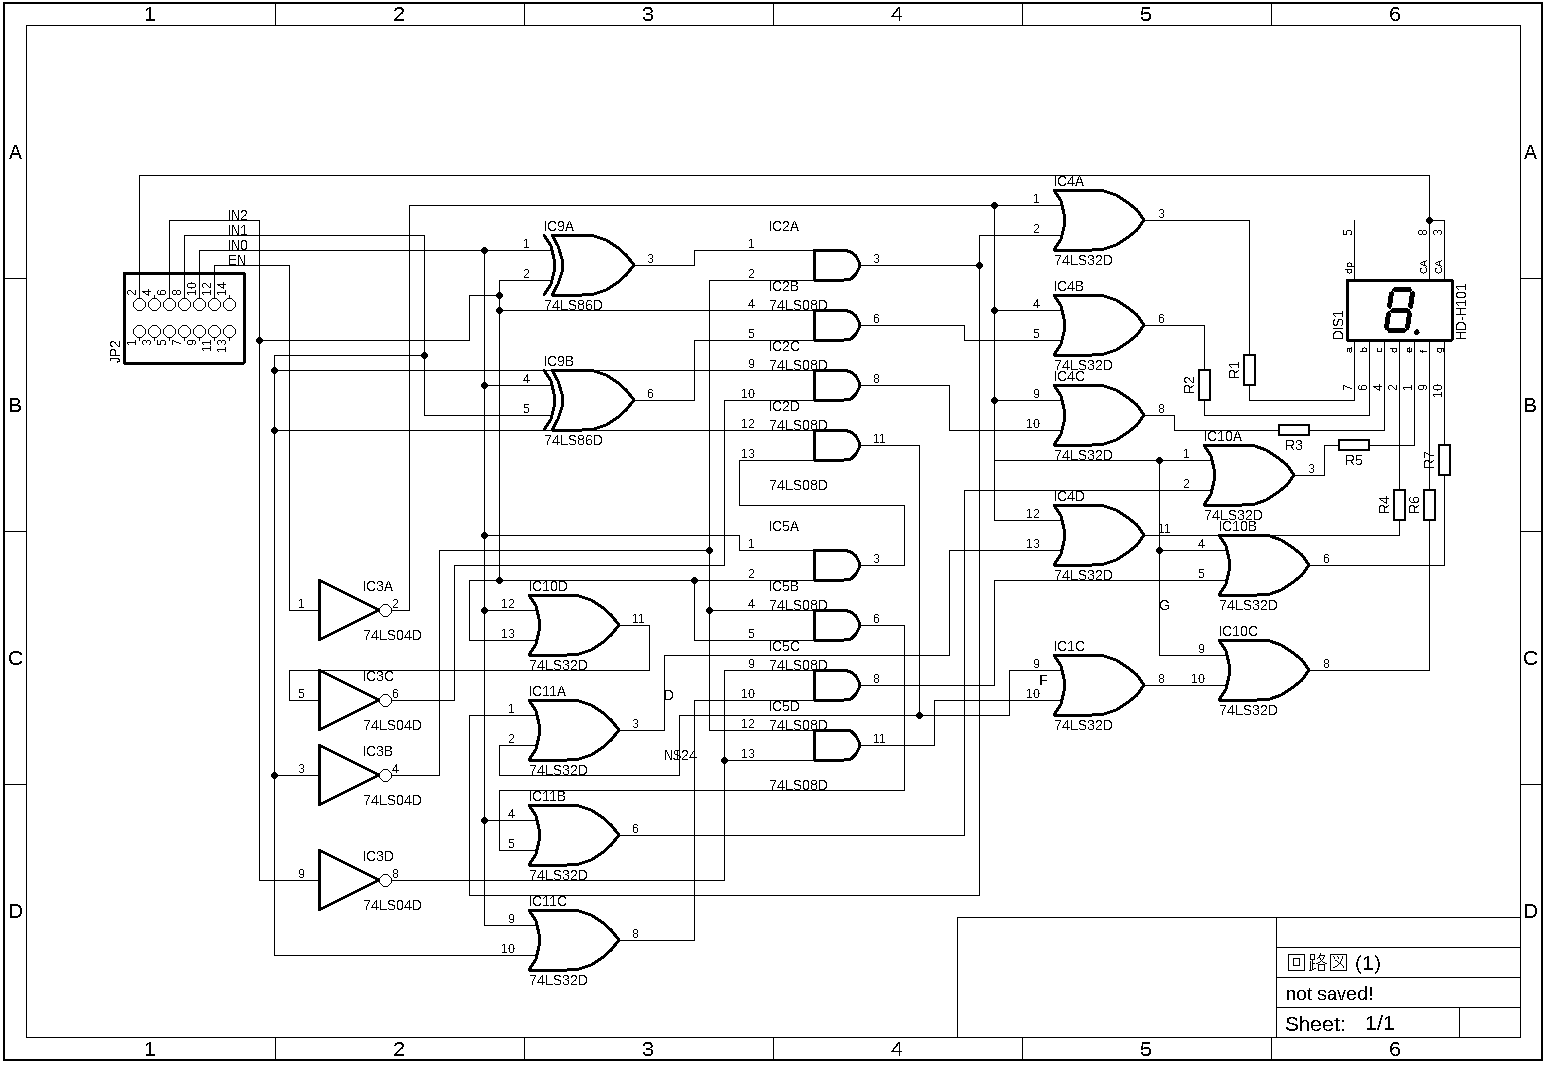
\includegraphics[width=15cm]{./images/circit.png}
  \caption{回路図}
  \label{fig:circit}
\end{figure}
\subsection{ブレッドボードへの配線}
作成した回路図を基にブレッドボードへの配線を行う。
実際に行った配線を図\ref{fig:haisen}に示す。
\begin{figure}[h]
  \centering
  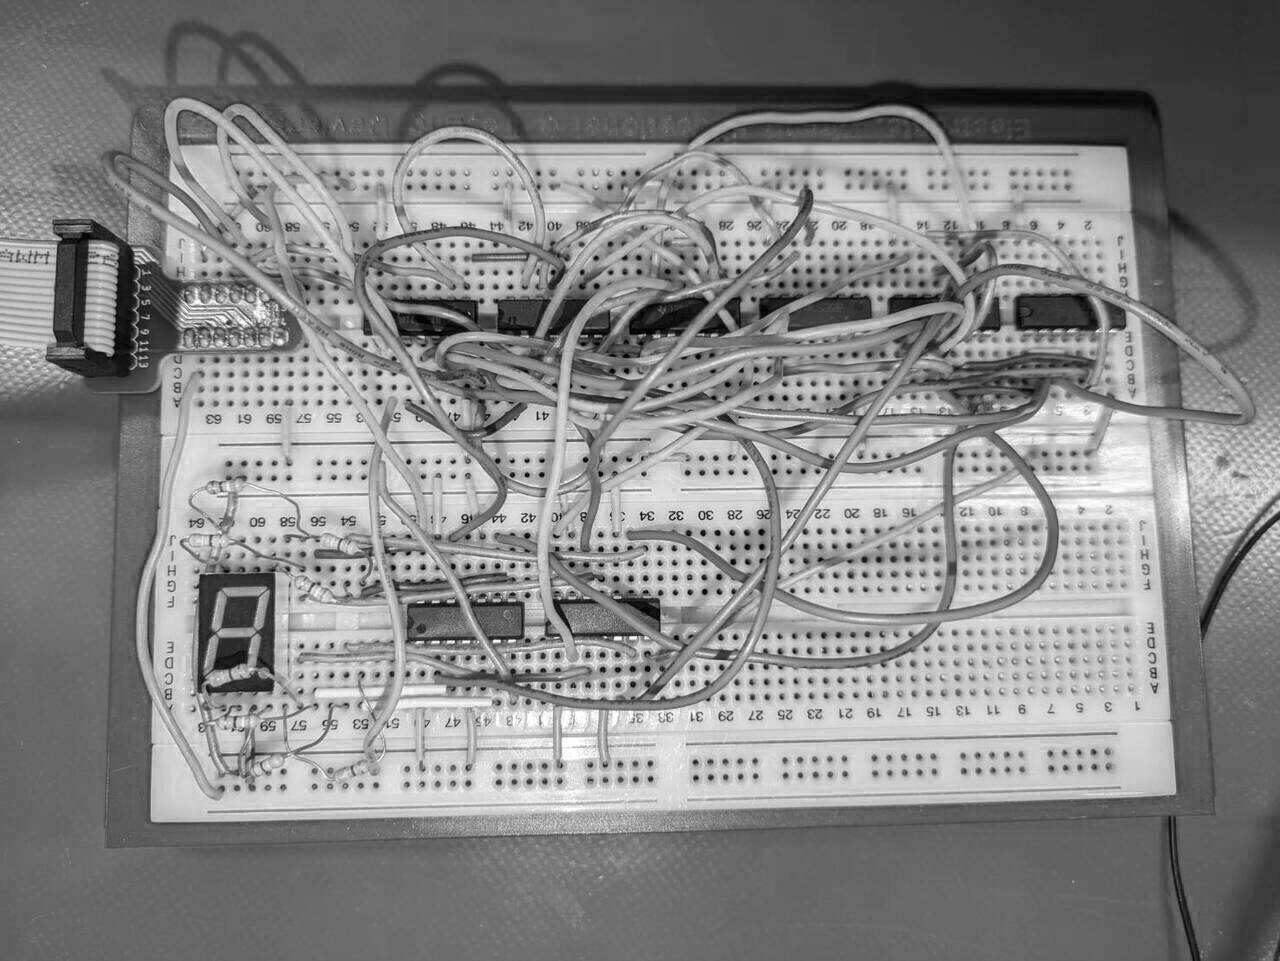
\includegraphics[width=15cm]{./images/haisen_gray.jpg}
  \caption{ブレッドボード}
  \label{fig:haisen}
\end{figure}

\section{結果}
作成した回路を動作させたところ、正常に動作した。
入力信号に応じて7セグLEDの表示が変わることが確認できた。

\section{考察}
今回の実験では、デコーダ回路を作成することで、ICを使った回路
の作成方法を学ぶことができた。また1から回路図を製作するにあたって、
真理値表やカルノー図を用いて論理式を作成する方法を学ぶことができた。
また今回は1度回路の組み立てを失敗してしまったため、丁寧にミスが
ないように配線を行うことの重要性を学ぶことができた。


\section{報告事項}
報告事項を以下に示す。

\begin{enumerate}
  \label{tab:ReportContents}
  \item $VCC=5$[V]の電源を使って$I_F=8$[mA]、$V_F=1.98$[V]のLEDを適切に光らせるために、必要な抵抗の値を求めて報告する。
  \item バイポーラトランジスタとCMOSの特徴を調べて報告する。
  \item ファンイン、ファンアウトについて調べて報告する。
  \item デコーダ回路の真理値表を作成し、報告する。
  \item セグメントBからGまでの論理式をたてて報告する。
  \item セグメントBからGまでの論理式をカルノー図を示しつつ、簡単化して報告する。
  \item 各セグメントを簡単化した論理式に基づき、セグメントBからGまでの回路図を作成して報告する。
  \item 7セグメントLEDおよび抵抗を含めたすべてのセグメントをまとめた回路図を描いて報告する。
\end{enumerate}

\subsection{報告事項a}
抵抗値はオームの法則より、$\frac{VCC-V_F}{I_F}$で求めることができる。
それぞれ$VCC=5$[V]、$I_F=8$[mA]、$V_F=1.98$[V]と与えられているので、$\frac{5-1.98(V)}{0.008(A)}=377.5\Omega$となり、LEDを適切に光らせるために必要な抵抗値は377.5$\Omega$と求めることができる。

\subsection{報告事項b}
バイポーラトランジスタの特徴を以下に示す。

\begin{enumerate}
  \item エミッタ(E)、ベース(B)、コレクタ(C)の3つの電極を持つ三端子素子。
  \item 主にアナログ集積回路で使用される。
  \item P型半導体、N型半導体を使用したPNP型、NPN型が存在する。
  \item PN接合の特徴を使って動作している。(逆方向バイアス、順方向バイアス)
  \item NPN型を例にすると、EをN型、BをP型、CをN型半導体がそれぞれの役割を果たしている。
\end{enumerate}
\cite{Khoritsu}、\cite{Ohmsha}より引用。\\

CMOSの特徴を以下に示す。

\begin{enumerate}
  \item 消費電力が少ない。
  \item 高入力・低出力インピーダンスである。
  \item 動作電圧範囲が広い。
  \item ノイズマージンが大きい。
  \item 温度特性が良い。
  \item 工程が複雑なため集積度が低い。
  \item 放熱の考慮が不必要である。
\end{enumerate}
\cite{DenkiDai}より引用。\\

\subsection{報告事項c}
論理ゲートの出力に次の段の論理ゲートの入力が接続されると、電流が流れる。
そして、出力のHighレベル、Lowレベルの電圧が変化する。\\
このとき、電圧が規格の最小値や最大値を超えないようにするために、
接続できる論理ゲートの数には上限がある。
この上限をそれぞれファンアウト、ファンインという。\\
ファンアウトとは、出力に接続可能な論理ゲート数の上限のことであり、
ファンインとは、入力に接続可能な論理ゲート数の上限のことである\cite{ShokoDo}。

\subsection{報告事項d}
表\ref{tab:truth}参照。

\subsection{報告事項e}
式(\ref{eq:a-output})、(\ref{eq:b-output})、(\ref{eq:c-output})、(\ref{eq:d-output})、(\ref{eq:e-output})、(\ref{eq:f-output})、(\ref{eq:g-output})参照。

\subsection{報告事項f}
カルノー図については図\ref{fig:karnoA}、\ref{fig:karnoB}、\ref{fig:karnoC}、
\ref{fig:karnoD}、\ref{fig:karnoE}、\ref{fig:karnoF}、
\ref{fig:karnoG}参照。\\
簡単かした論理式については式(\ref{eq:a-output1})、(\ref{eq:b-output1})、
(\ref{eq:c-output})、(\ref{eq:d-output1})、(\ref{eq:e-output})、
(\ref{eq:f-output1})、(\ref{eq:g-output})参照。

\subsection{報告事項g}
セグメントBからGまでの回路図を示す。
\subsubsection{セグメントB}
セグメントBの回路図を図\ref{fig:segmentB}に示す。
\begin{figure}[H]
  \centering
  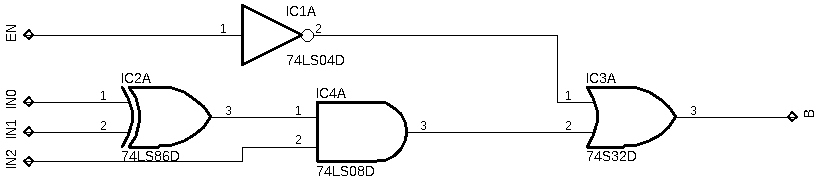
\includegraphics[width=10cm]{./images/B.png}
  \caption{セグメントBの回路図}
  \label{fig:segmentB}
\end{figure}

\subsubsection{セグメントC}
セグメントCの回路図を図\ref{fig:segmentC}に示す。
\begin{figure}[H]
  \centering
  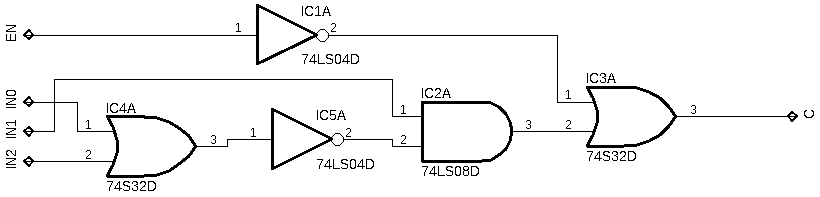
\includegraphics[width=10cm]{./images/C.png}
  \caption{セグメントCの回路図}
  \label{fig:segmentC}
\end{figure}

\subsubsection{セグメントD}
セグメントDの回路図を図\ref{fig:segmentD}に示す。
\begin{figure}[H]
  \centering
  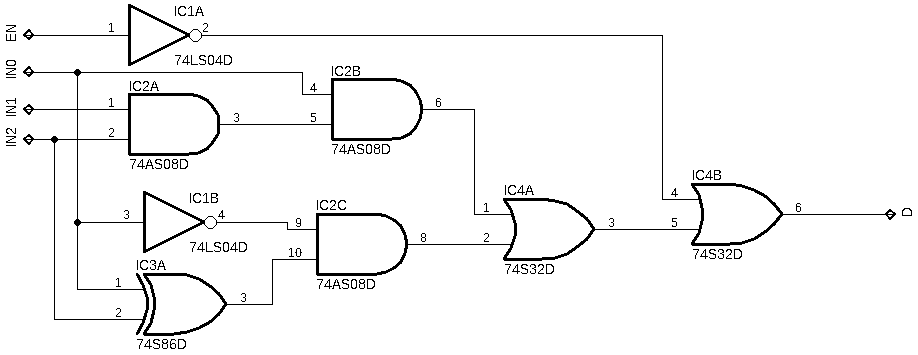
\includegraphics[width=10cm]{./images/D.png}
  \caption{セグメントDの回路図}
  \label{fig:segmentD}
\end{figure}

\subsubsection{セグメントE}
セグメントEの回路図を図\ref{fig:segmentE}に示す。
\begin{figure}[H]
  \centering
  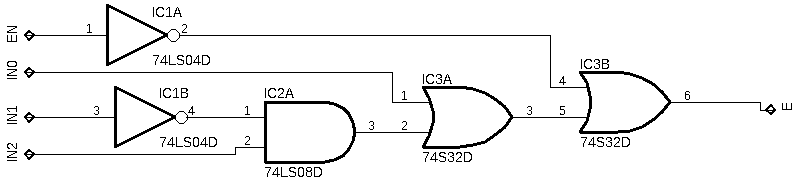
\includegraphics[width=10cm]{./images/E.png}
  \caption{セグメントEの回路図}
  \label{fig:segmentE}
\end{figure}

\subsubsection{セグメントF}
セグメントFの回路図を図\ref{fig:segmentF}に示す。
\begin{figure}[H]
  \centering
  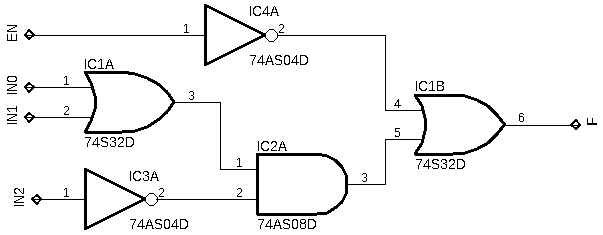
\includegraphics[width=10cm]{./images/F.png}
  \caption{セグメントFの回路図}
  \label{fig:segmentF}
\end{figure}

\subsubsection{セグメントG}
セグメントGの回路図を図\ref{fig:segmentG}に示す。
\begin{figure}[H]
  \centering
  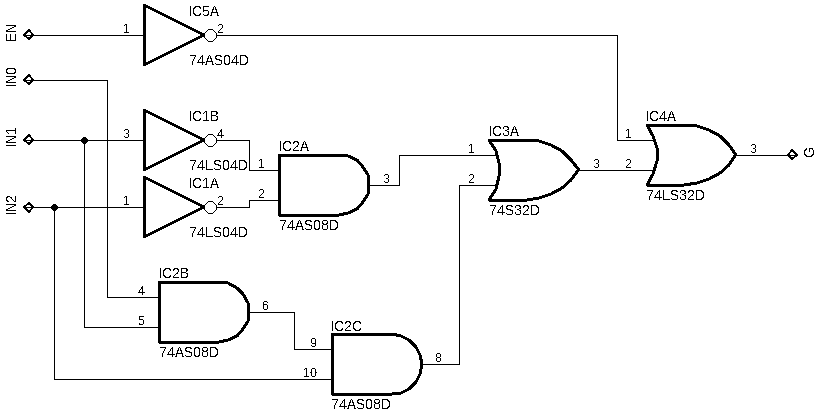
\includegraphics[width=10cm]{./images/G.png}
  \caption{セグメントGの回路図}
  \label{fig:segmentG}
\end{figure}

\subsection{報告事項h}
図\ref{fig:circit}参照。

\addcontentsline{toc}{section}{参考文献}
\begin{thebibliography}{99}
  \bibitem{Khokasho} 浜辺 隆二 著,『論理回路入門 第4版』、森北出版、p84、2022年
  \bibitem{Khoritsu} 宮入圭一 監修、阿部勝也 著、『本質を学ぶためのアナログ電子回路入門』、共立出版、pp.30-31、2007年
  \bibitem{Ohmsha} 藤井信夫 著、『アナログ電子回路-集積回路化時代の-』、オーム社、pp.20-22、2014年
  \bibitem{DenkiDai} 岩崎臣男 監修、赤羽進/山本敏正/高坪守男/板倉利行/臼井秀司 共著、『解説ICの基礎3訂番』、東京電機大出版局、p34、1996年
  \bibitem{ShokoDo} 藤井信夫 著、『集積回路化時代のディジタル電子回路』、昭晃堂、pp.50-63、1987年
\end{thebibliography}

\end{document}